\clearpage
\cleardoublepage

\chapter{Core Operations in Neural Networks}

\section{Introduction}

This chapter covers the fundamental building blocks of modern neural networks: convolution, pooling, and normalization operations. Understanding these operations is essential for designing and implementing effective neural network architectures.

\section{Convolution Operation}

Convolution is the cornerstone of convolutional neural networks (CNNs).

\subsection{2D Convolution}

For input $\mathbf{X} \in \mathbb{R}^{H \times W}$ and kernel $\mathbf{K} \in \mathbb{R}^{K \times K}$:
\begin{equation}
y[i,j] = \sum_{m=0}^{K-1}\sum_{n=0}^{K-1} k[m,n] \cdot x[i+m, j+n]
\end{equation}

In practice, we often add bias and use multiple kernels for multiple output channels.

\begin{properties}[Convolution Parameters]
\begin{itemize}
    \item \textbf{Kernel size:} $K \times K$ (common: $3\times3$, $5\times5$, $7\times7$)
    \item \textbf{Stride ($s$):} Step size for sliding window
    \item \textbf{Padding ($p$):} Zero padding around input
    \item \textbf{Dilation ($d$):} Spacing between kernel elements
\end{itemize}
\end{properties}

Output size with padding and stride:
\begin{equation}
H_{out} = \left\lfloor \frac{H_{in} + 2p - d(K-1) - 1}{s} + 1 \right\rfloor
\end{equation}

\begin{figure}[htbp]
    \centering
    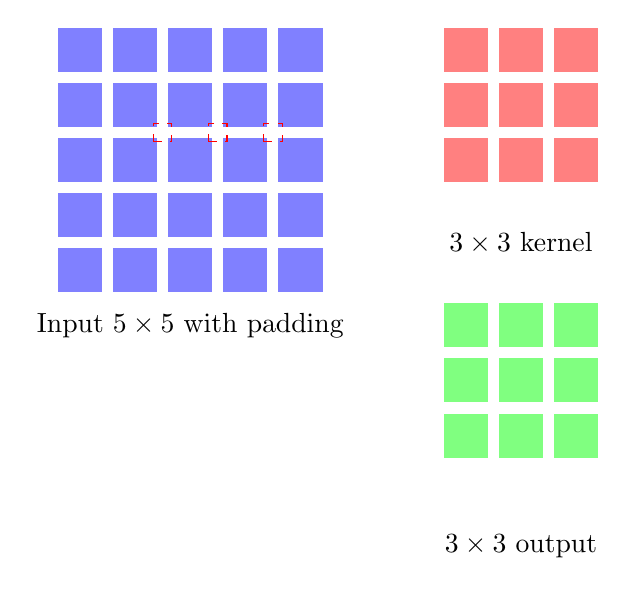
\begin{tikzpicture}[scale=0.7]
        % Input with padding
        \foreach \x in {0,...,4} {
            \foreach \y in {0,...,4} {
                \ifthenelse{\x < 1 \OR \x > 3 \OR \y < 1 \OR \y > 3}
                {\fill[gray!30] (\x, \y) +(-0.4, -0.4) rectangle ++(0.4, 0.4);}
                {\fill[blue!50] (\x, \y) +(-0.4, -0.4) rectangle ++(0.4, 0.4);}
            }
        }
        \node at (2, -1) {Input $5\times5$ with padding};
        
        % Kernel
        \foreach \x in {0,...,2} {
            \foreach \y in {0,...,2} {
                \fill[red!50] (7+\x, 2+\y) +(-0.4, -0.4) rectangle ++(0.4, 0.4);
            }
        }
        \node at (8, 0.5) {$3\times3$ kernel};
        
        % Output
        \foreach \x in {0,...,2} {
            \foreach \y in {0,...,2} {
                \fill[green!50] (7+\x, -3+\y) +(-0.4, -0.4) rectangle ++(0.4, 0.4);
            }
        }
        \node at (8, -5) {$3\times3$ output};
        
        % Stride 1
        \node[draw, dashed, red] at (1.5, 2.5) {};
        \node[draw, dashed, red] at (2.5, 2.5) {};
        \node[draw, dashed, red] at (3.5, 2.5) {};
    \end{tikzpicture}
    \caption{Convolution with padding}
    \label{fig:conv_padding}
\end{figure}

\subsection{Grouped and Depthwise Convolution}

\begin{itemize}
    \item \textbf{Grouped convolution:} Split input channels into groups, apply separate conv per group
    \item \textbf{Depthwise convolution:} One kernel per input channel (grouped with $G = C_{in}$)
    \item \textbf{Pointwise convolution:} $1\times1$ conv (used to mix channels)
\end{itemize}

MobileNet uses: Depthwise Separable Convolution = Depthwise + Pointwise

\begin{properties}[Depthwise Separable Convolution]
\begin{itemize}
    \item \textbf{Standard conv FLOPs:} $H \cdot W \cdot K^2 \cdot C_{in} \cdot C_{out}$
    \item \textbf{Separable conv FLOPs:} $H \cdot W \cdot K^2 \cdot C_{in} + H \cdot W \cdot C_{in} \cdot C_{out}$
    \item \textbf{Speedup:} $\frac{1}{K^2} + \frac{1}{C_{out}}$ approximately
\end{itemize}
\end{properties}

\subsection{Dilated (Atrous) Convolution}

Dilated convolution inserts zeros between kernel elements, expanding the receptive field without increasing the parameter count or computation:

\begin{equation}
y[i,j] = \sum_{m=0}^{K-1}\sum_{n=0}^{K-1} k[m,n] \cdot x[i + m \cdot d, j + n \cdot d]
\end{equation}
where $d$ is the dilation rate.

\begin{properties}[Dilated Convolution Properties]
\begin{itemize}
    \item \textbf{Receptive field with dilation $d$:} Effective kernel size $= d(K - 1) + 1$
    \item \textbf{FLOPs:} Same as standard convolution (only the sampling pattern changes)
    \item \textbf{Parameters:} Same as standard convolution
    \item \textbf{Key application:} Semantic segmentation (DeepLab series), where large receptive fields are needed without pooling or striding
\end{itemize}
\end{properties}

\begin{example}[Stacked Dilated Convolutions]
Three $3 \times 3$ convolutions with dilation rates $d = 1, 2, 4$ produce a total receptive field of:
\begin{equation}
\text{RF} = 1 + (3-1)\times1 + (3-1)\times2 + (3-1)\times4 = 15
\end{equation}
This matches a $15 \times 15$ standard convolution but with only $3 \times 9C^2$ parameters instead of $225C^2$. This is the core idea behind \textbf{DeepLab} (Chen et al., 2017).
\end{example}

\section{Pooling Operations}

Pooling reduces spatial dimensions and provides translation invariance.

\subsection{Max Pooling}

\begin{equation}
y[i,j] = \max_{m,n \in \mathcal{N}(i,j)} x[m,n]
\end{equation}

where $\mathcal{N}(i,j)$ is the neighborhood.

\begin{itemize}
    \item \textbf{Retains strongest activation}
    \item \textbf{Provides local translation invariance}
    \item \textbf{Common: } $2\times2$ with stride 2
\end{itemize}

\subsection{Average Pooling}

\begin{equation}
y[i,j] = \frac{1}{K \cdot K}\sum_{m,n \in \mathcal{N}(i,j)} x[m,n]
\end{equation}

\begin{itemize}
    \item \textbf{Averages over neighborhood}
    \item \textbf{Less aggressive than max pooling}
    \item \textbf{Used in global pooling}
\end{itemize}

\begin{figure}[htbp]
    \centering
    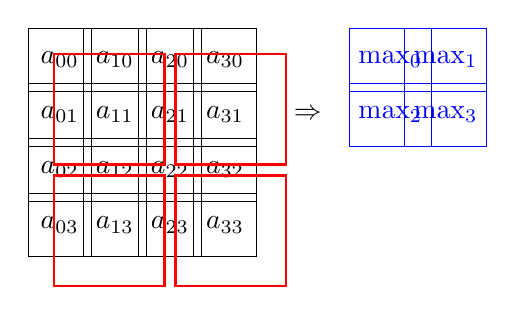
\begin{tikzpicture}[scale=0.7]
        % Input
        \foreach \x in {0,...,3} {
            \foreach \y in {0,...,3} {
                \node[draw, minimum size=0.8cm] at (\x, -\y) {$a_{\x\y}$};
            }
        }
        
        % Max pooling boxes
        \draw[red, thick] (-0.1, 0.1) rectangle (1.9, -1.9);
        \draw[red, thick] (2.1, 0.1) rectangle (4.1, -1.9);
        \draw[red, thick] (-0.1, -2.1) rectangle (1.9, -4.1);
        \draw[red, thick] (2.1, -2.1) rectangle (4.1, -4.1);
        
        \node at (4.5, -1) {$\Rightarrow$};
        
        % Output
        \node[draw, blue, minimum size=0.8cm] at (6, 0) {$\max_0$};
        \node[draw, blue, minimum size=0.8cm] at (7, 0) {$\max_1$};
        \node[draw, blue, minimum size=0.8cm] at (6, -1) {$\max_2$};
        \node[draw, blue, minimum size=0.8cm] at (7, -1) {$\max_3$};
    \end{tikzpicture}
    \caption{Max pooling $2\times2$, stride 2}
    \label{fig:maxpool}
\end{figure}

\subsection{Global Pooling}

Applied over entire feature map to produce single value per channel:
\begin{itemize}
    \item \textbf{Global Average Pooling (GAP):} $\frac{1}{HW}\sum_{i,j} x_{ij}$
    \item \textbf{Global Max Pooling:} $\max_{i,j} x_{ij}$
    \item \textbf{Replaces FC layers} in modern architectures
\end{itemize}

\section{Normalization Techniques}

Normalization stabilizes training by controlling layer input distributions.

\subsection{Batch Normalization}

Normalizes activations across batch dimension:
\begin{equation}
\hat{x}_i = \frac{x_i - \mu_B}{\sqrt{\sigma_B^2 + \epsilon}}, \quad y_i = \gamma \hat{x}_i + \beta
\end{equation}

where:
\begin{align}
\mu_B &= \frac{1}{m}\sum_{i=1}^{m} x_i \\
\sigma_B^2 &= \frac{1}{m}\sum_{i=1}^{m}(x_i - \mu_B)^2
\end{align}

\begin{properties}[BatchNorm Properties]
\begin{itemize}
    \item \textbf{Reduces internal covariate shift}
    \item \textbf{Allows higher learning rates}
    \item \textbf{Provides slight regularization}
    \item \textbf{Dependent on batch size and can be problematic in small batches}
\end{itemize}
\end{properties}

\begin{note}[BatchNorm vs. Inference]
During training, BatchNorm uses batch statistics. During inference, use running statistics:
\begin{equation}
\hat{x} = \frac{x - \tilde{\mu}}{\sqrt{\tilde{\sigma}^2 + \epsilon}}
\end{equation}
where $\tilde{\mu}$ and $\tilde{\sigma}^2$ are running averages.
\end{note}

\subsection{Layer Normalization}

Normalizes across features within a single sample:
\begin{equation}
\mu = \frac{1}{D}\sum_{i=1}^{D} x_i, \quad \sigma = \frac{1}{D}\sum_{i=1}^{D}(x_i - \mu)^2
\end{equation}

\begin{itemize}
    \item \textbf{Independent of batch size}
    \item \textbf{Used in RNNs and Transformers}
    \item \textbf{Same for training and inference}
\end{itemize}

\begin{table}[ht]
    \centering
    \caption{Normalization Comparison}
    \begin{tabular}{L{2cm} L{2.5cm} L{2.5cm} L{3cm}}
        \toprule
        \textbf{Method} & \textbf{Normalize over} & \textbf{Batch dep.} & \textbf{Use case} \\
        \midrule
        BatchNorm & $(H, W, C)$ & Yes & CNNs \\
        LayerNorm & $(H, W, N)$ & No & Transformers \\
        InstanceNorm & $(H, W)$ & No & Style transfer \\
        GroupNorm & $(H, W, G)$ & No & Small batch CNNs \\
        \bottomrule
    \end{tabular}
\end{table}

\subsection{Instance Normalization}

Normalizes each sample and channel independently:
\begin{equation}
y_{nchw} = \frac{x_{nchw} - \mu_{nc}}{\sqrt{\sigma_{nc}^2 + \epsilon}}
\end{equation}

Used in style transfer where instance-specific statistics matter.

\subsection{Group Normalization}

Group Normalization (GN) divides channels into $G$ groups and normalizes within each group independently (Wu \& He, 2018). This provides a unified framework that subsumes LayerNorm and InstanceNorm as special cases.

For a tensor of shape $(N, C, H, W)$ with $C/G$ channels per group:
\begin{align}
\mu_g &= \frac{1}{(C/G) \cdot H \cdot W} \sum_{c \in \mathcal{G}_g} \sum_{h,w} x_{nchw} \\
\sigma_g^2 &= \frac{1}{(C/G) \cdot H \cdot W} \sum_{c \in \mathcal{G}_g} \sum_{h,w} (x_{nchw} - \mu_g)^2 \\
\hat{x}_{nchw} &= \frac{x_{nchw} - \mu_g}{\sqrt{\sigma_g^2 + \epsilon}}
\end{align}

\begin{properties}[GN as a Unified Framework]
\begin{itemize}
    \item $G = 1$: GroupNorm becomes \textbf{LayerNorm} (normalize across all channels)
    \item $G = C$: GroupNorm becomes \textbf{InstanceNorm} (normalize per-channel)
    \item $G = 32$ is the default in most implementations (a good tradeoff)
    \item \textbf{Independent of batch size}: works with batch size 1 (e.g., in medical imaging)
    \item Computationally equivalent to BatchNorm; only the grouping changes
\end{itemize}
\end{properties}

\begin{table}[ht]
    \centering
    \caption{Normalization Methods: Unified View}
    \begin{tabular}{L{2cm} L{3cm} L{2cm} L{3.5cm}}
        \toprule
        \textbf{Method} & \textbf{Compute stats over} & \textbf{Batch dep.} & \textbf{Primary use} \\
        \midrule
        BatchNorm & $(N, H, W)$ per $C$ & Yes & CNNs (large batch) \\
        LayerNorm & $(H, W, C)$ per $N$ & No & Transformers, RNNs \\
        InstanceNorm & $(H, W)$ per $N,C$ & No & Style transfer \\
        GroupNorm & $(H, W, C/G)$ per $N$ & No & Detection, small batch \\
        \bottomrule
    \end{tabular}
\end{table}

\section{Regularization Operations}

Beyond normalization, several operations prevent overfitting by introducing stochasticity or constraints during training.

\subsection{Dropout}

Dropout (Srivastava et al., 2014) randomly sets activations to zero during training with probability $p$:
\begin{equation}
\tilde{x}_i = \frac{m_i \cdot x_i}{1 - p}, \quad m_i \sim \text{Bernoulli}(1 - p)
\end{equation}
The scaling factor $1/(1-p)$ (inverted dropout) ensures that $\mathbb{E}[\tilde{x}_i] = x_i$, so no adjustment is needed at inference.

\subsubsection{Why Dropout Works: Bayesian Interpretation}

Dropout can be viewed as approximate Bayesian inference (Gal \& Ghahramani, 2016). Each dropout mask defines a different sub-network, and training with dropout is equivalent to:
\begin{equation}
p(\mathbf{y} \mid \mathbf{x}, \mathcal{D}) \approx \frac{1}{T}\sum_{t=1}^{T} p(\mathbf{y} \mid \mathbf{x}, \mathbf{W} \odot \mathbf{m}^{(t)})
\end{equation}
This is \textbf{model averaging} over an exponential number of thinned networks ($2^N$ for $N$ units), which reduces variance and improves generalization.

\subsubsection{Variants of Dropout}

\begin{table}[ht]
    \centering
    \caption{Dropout Variants}
    \begin{tabular}{L{3cm} L{4.5cm} L{4.5cm}}
        \toprule
        \textbf{Variant} & \textbf{Operation} & \textbf{Use Case} \\
        \midrule
        Standard Dropout & Zero activations with prob.\ $p$ & FC layers \\
        DropConnect & Zero \textit{weights} with prob.\ $p$ & FC layers \\
        Spatial Dropout & Drop entire feature maps & CNNs \\
        DropPath & Skip entire path/blocks & Deep networks \\
        DropBlock & Drop contiguous regions & CNNs (regularization) \\
        \bottomrule
    \end{tabular}
\end{table}

\textbf{DropPath} (Stochastic Depth, Huang et al., 2016) randomly skips entire residual blocks during training. For a block with input $\mathbf{x}$ and output $\mathcal{F}(\mathbf{x})$:
\begin{equation}
\tilde{\mathbf{y}} = \begin{cases} \mathbf{x} & \text{with probability } p_L \\ \mathcal{F}(\mathbf{x}) + \mathbf{x} & \text{with probability } 1 - p_L \end{cases}
\end{equation}
The drop rate $p_L$ typically increases linearly with depth, creating shorter effective networks during training that act as an ensemble.

\section{Combining Operations}

Modern networks combine these operations in standardized blocks.

\subsection{Basic Conv Block}

A typical convolutional block:
\begin{enumerate}
    \item Convolution
    \item Batch Normalization
    \item Activation (ReLU/GELU)
\end{enumerate}

Common patterns:
\begin{itemize}
    \item Conv-BN-ReLU (VGG style)
    \item BN-ReLU-Conv (ResNet style, pre-activation)
\end{itemize}

\begin{code}
    \captionof{listing}{Conv Block in PyTorch}
    \label{code:conv_block}
\begin{lstlisting}[language=python]
import torch.nn as nn

class ConvBlock(nn.Module):
    def __init__(self, in_ch, out_ch, kernel_size=3, stride=1):
        super().__init__()
        padding = kernel_size // 2
        self.block = nn.Sequential(
            nn.Conv2d(in_ch, out_ch, kernel_size, stride, padding, bias=False),
            nn.BatchNorm2d(out_ch),
            nn.ReLU(inplace=True)
        )
    
    def forward(self, x):
        return self.block(x)

# Pre-activation block (ResNet style)
class PreActBlock(nn.Module):
    def __init__(self, in_ch, out_ch, stride=1):
        super().__init__()
        self.block = nn.Sequential(
            nn.BatchNorm2d(in_ch),
            nn.ReLU(inplace=True),
            nn.Conv2d(in_ch, out_ch, 3, stride, 1, bias=False),
            nn.BatchNorm2d(out_ch),
            nn.ReLU(inplace=True),
            nn.Conv2d(out_ch, out_ch, 3, 1, 1, bias=False)
        )
        self.shortcut = nn.Identity() if stride==1 and in_ch==out_ch else \
                        nn.Conv2d(in_ch, out_ch, 1, stride, bias=False)
    
    def forward(self, x):
        return self.block(x) + self.shortcut(x)
\end{lstlisting}
\end{code}

\section{Chapter Summary}

\begin{enumerate}
    \item Convolution extracts local features with shared weights
    \item Depthwise separable convolution reduces computation for mobile deployment
    \item Dilated convolution expands receptive field without extra parameters
    \item Pooling provides spatial reduction and invariance
    \item Normalization stabilizes training dynamics (BN for CNNs, LN for Transformers, GN for small batches)
    \item Dropout and its variants provide regularization through stochastic depth
    \item Modern architectures combine these in standardized blocks
    \item Choice of operations depends on task and data characteristics
\end{enumerate}

\section{Further Reading}

\begin{itemize}
    \item Ioffe, S. \& Szegedy, C. (2015). Batch normalization: Accelerating deep network training by reducing internal covariate shift. \textit{ICML}.
    \item Ba, J., Kiros, J., \& Hinton, G. (2016). Layer normalization. \textit{arXiv:1607.06450}.
    \item Wu, Y. \& He, K. (2018). Group normalization. \textit{ECCV}.
    \item Srivastava, N. et al. (2014). Dropout: A simple way to prevent neural networks from overfitting. \textit{JMLR}, 15, 1929--1958.
    \item Gal, Y. \& Ghahramani, Z. (2016). Dropout as a Bayesian approximation: Representing model uncertainty in deep learning. \textit{ICML}.
    \item Huang, G. et al. (2016). Deep networks with stochastic depth. \textit{ECCV}.
    \item Chen, L.-C. et al. (2017). Rethinking atrous convolution for semantic image segmentation. \textit{arXiv:1706.05587}.
    \item Howard, A. et al. (2017). MobileNets: Efficient convolutional neural networks for mobile vision applications. \textit{arXiv:1704.04861}.
\end{itemize}
